\documentclass{standalone}
\usepackage[T1]{fontenc}
\usepackage[latin2]{inputenc}
\usepackage[english]{babel}
\usepackage{tikz}
\usepackage{times}
\usetikzlibrary{calc,through,backgrounds,positioning,fit}
\usetikzlibrary{shapes,arrows,shadows,calendar}
\begin{document}

\begin{tikzpicture}
\node (A) at(-3,-1.5)   {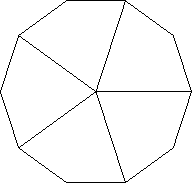
\includegraphics[scale=1]{10a.pdf}};
\node (B) at( 3,-1.5)   {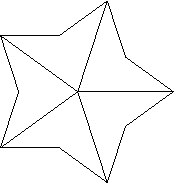
\includegraphics[scale=1]{10b.pdf}};
\node (C) at(-3, 1.5) {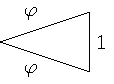
\includegraphics[scale=1]{10c.pdf}};
\node (D) at( 3, 1.5)  {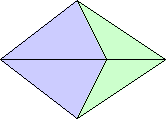
\includegraphics[scale=1]{10d.pdf}};
\end{tikzpicture}
\end{document}